% -*- root: These.tex -*-

\section{Simprocess}
\label{sec:simprocess}

\subsection{Le système de workflow OpenMOLE}

\subsubsection{Historique}

\subsubsection{Principes et mise en oeuvre}

\subsection{Algorithmes Evolutionnaire}

% Présentation de l'interet de ces techniques

Pour mieux comprendre par la suite quel est la spécificité des algorithmes evolutionnaires (\textit{Evolutionary Algorithms} ou EA), il est nécessaire de donner quelques éléments de contexte et de définitions plus généraux concernant la branche d'étude dans lequel ceux-ci se situent. Il faut par ailleurs mettre en garde le lecteur que la plupart des définitions présentés ici sont extraites d'ouvrages de synthèses à destination d'un public très large \autocites{Weise2011, Luke2013, Brownlee2012}. Par conséquent il faut garder à l'esprit que plusieurs de ces termes peuvent être discutés, enrichis ou critiqués (quand il existe !) dans chacune des sous branche (voir figure \ref{fig:S_OverviewOptimisation}) que compte ce domaine très général qu'est l'optimisation.

\begin{figure}[h]
\begin{sidecaption}[fortoc]{ Vue d'ensemble des algorithmes d'optimisation repris de l'état de l'art très complet de \textcite[32]{Weise2011}}[fig:S_OverviewOptimisation]
  \centering
 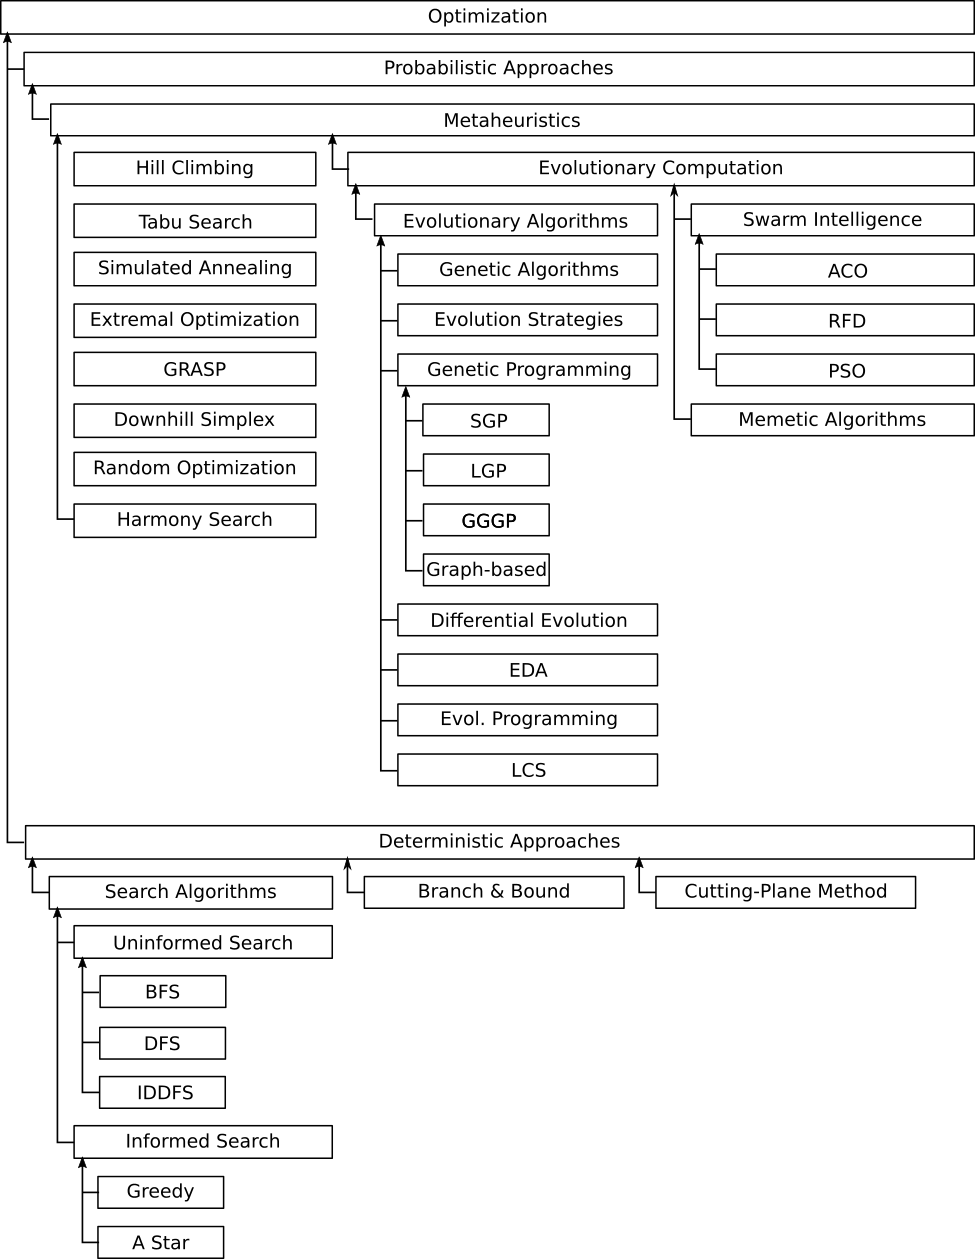
\includegraphics[width=.9\linewidth]{overview_optimisation_algorithm.png}
  \end{sidecaption}
\end{figure}

\subsubsection{Le domaine des algorithmes métaheuristiques, une sous-discipline de l'Optimisation}

\paragraph{Q'est ce que l'optimisation ?}

Pour \textcite[22]{Weise2011}, l'optimisation \foreignquote{english}{ [...] is the process of solving an optimization problem, i. e., finding suitable solutions for it}, un problème d'optimisation nécessitant de trouver \foreignquote{english}{ [...] an input value $x^*$ for which a mathematical function $f$ takes on the smallest possible value (while usually obeying to some restrictions on the possible values of $x^*$ )}.

Sortie de cette définition mathématique, l'optimisation peut également se définir par la mise en oeuvre d'algorithmes spécifiques. La littérature informatique met à disposition des programmeurs un ensemble d'algorithmes capables de fournir des solutions exactes dans un temps fini à un certain nombre de problèmes bien définis. C'est le cas par exemple des nombreux algorithmes de tri. Une autre classe d'algorithmes (\textit{optimization algorithms}) peut être employée lorsqu'il n'existe pas d'algorithme dédié (\textit{dedicated algorithms}), soit parce que le problème est trop spécifique, soit parce que personne n'a trouvé de solution efficace pour résoudre ce problème. 

Dans ce cadre, le terme d'optimisation globale \foreignquote{english}{ [...] is optimization with the goal of finding solutions $x^*$ for a given optimization problem which have the property that no other, better solutions exist.}

Bien que souvent beaucoup plus lent, moins précis, et plus consommateurs de ressources que les algorithmes du premier type, ces derniers nécessitent aussi beaucoup moins d'informations pour pouvoir être executés : \foreignquote{english}{Most often, these algorithms only need a definition of the structure of possible solutions and a function $f$ which tells measures the quality of a candidate solution. Based on this information, they try to find solutions for which $f$ takes on the best values.} \autocite[24]{Weise2011}

Ces algorithmes s'appuient donc sur différents types de stratégies pour tirer partie du peu d'information injecté via $f$. Ces dernières étant de nature très diverse, on retient ici une première typologie en deux classes pour les séparer. D'une coté les approches stochastiques (\textit{Probabilistic Approaches} dans la fig. \ref{fig:S_OverviewOptimisation}) sont capables de trouver un optimum assez rapidement, mais ne peuvent pas en garantir la propriété \enquote{globale}, et d'un autre coté certaines approches déterministes (\textit{Deterministic Approaches} dans la fig. \ref{fig:S_OverviewOptimisation}) qui peuvent certes garantir au moins théoriquement l'obtention d'un optimum global, mais au détriment souvent d'un coût computationnel elevé. Les deux approches partagent également des difficultés similaires, à des degrés divers, dès lors que l'espace de recherche devient trop important.

Cette typologie recoupe comme on le constate dans sa définition une autre propriété des algorithmes. On qualifie d'\textit{exact} les algorithmes dont l'exécution garantie un résultat optimum à coup sûr, d'\textit{approximate algorithms} les algorithmes capable de donner une mesure proche d'un optimum sans pouvoir en garantir la qualité, et d'\textit{approximation algorithms} les algorithmes capables de donner une mesure proche d'un optimum assorti d'une preuve de qualité. Cette dernière classe n'est pas à confondre avec une classe d'algorithmes cherchant à conserver l'optimalité en limitant par diverses stratégies le cout temporel de résolution, mais bien l'inverse, relacher la contrainte d'optimalité, mais aussi peu que possible. Les \textit{approximations algorithms} sont une donc une sous classe d'\textit{approximate algorithms}, et constitue une branche d'étude à eux seul, car même dans le cas de problèmes \textit{NP-Complet}, ils offrent dans des dimensions raisonnables et propres à chacun des problèmes une solution sub-optimale d'erreur mesurable et donc potentiellement améliorable, voire comparable, notamment avec les résultats donnés de façon non analytique par des heuristiques. 
%http://en.wikipedia.org/wiki/Approximation_algorithm#cite_ref-kann92onthe_3-4

On retrouve parfois rangé \enquote{en vrac} dans la classe des \textit{approximate algorithms} la classe des heuristiques et métaheuristiques - dont on définira le sens plus en détail dans la section suivante - mais cette typologie ne semble pas totalement juste non plus. Par exemple de multiples problèmes trouvent une solution exacte jusqu'à un certain niveau de complexification, à partir duquel on fait généralement appel aux heuristiques, soit par un appel à d'autres méthodes intégrant des heuristiques, soit par une intégration d'heuristiques aux méthodes existantes. Ainsi de nombreuses classes d'heuristiques sont utilisées de façon transversales, et apparaissent donc aussi comme composantes manipulées dans la classes des \textit{approximation algorithms}. L'heuristique glouton \textit{greedy algorithm} \Anote{greedy_description} apparait de façon transversale à la fois comme une solution d'approximation pour le \textit{Knapsack Problem} (KP) mais également comme moteur dans le cadre d'algorithmes déterministes exacts comme Djikstra. Un autre algorithme nommé \textit{A*} qui est un cas particulier de ce dernier est quant à lui capable de fournir tout à la fois une mesure exacte ou approximée en fonction de l'heuristique injectée et du niveau de complexité du problème abordé. Dernier exemple, si les méthodes métaheuristiques sont effectivement souvent connu pour ne pas avancer de preuve, des travaux récents montre toutefois qu'il existe de nouveaux algorithmes permettant de garantir dans certaines conditions un optimum global (CP-Algorithm de \autocite{Reuillon2014}). Tout dépend donc du degré et de la nature que l'on veut bien associer à la notion d'\textit{approximation} lorsqu'il s'agit de fournir une mesure d'éloignement de l'optimum. Les \textit{approximation algorithms} semblent toutefois plus intéressé par l'établissement d'une preuve au sens mathématique, et se concentre avant tout sur un ensemble relativement limité de problèmes d'optimisation discret, ce qui ne semble pas être le but des métaheuristiques dans les deux cas. \autocite[1-6]{Kann1992} \autocite[13-15]{Williamson2011} %Metaheuristics: From Design to Implementation Par El-Ghazali Talbi

%You could think of a heuristic like an approximate (not approximation) solution to a problem. The difference between approximate and approximation is that the first is about getting a good guess of the solution of a problem, but that you don't really know how good it is. The second is about getting a solution for which you can prove how close it is to the optimal solution.

Enfin bien d'autres sous classifications sont possibles prenant plus ou moins en compte les spécificités propres aux différents algorithmes, comme celle opposant par exemple les stratégies utilisées en interne pour parcourir l'espace de recherche (generationel vs steady-state, ou individuel vs populationel), la dimensionnalité possible pour la résolution des problèmes (mono-objectif vs multi-objectif), l'inspiration d'origine (naturelle biologique vs autres), etc. 

Toute classification monocritère est donc rendue très difficile, une voie s'étant même ouverte pour tenter de classifier ces algorithmes suivant la nature et le niveau d'opération de ces hybridations. L'origine de cette difficulté tient dans une pratique courante et assumée d'hybridation entre les différentes techniques afin de réunir le meilleur de chacune d'elle au sein de nouvelle proposition de recherche. De fait, il est important pour la suite de cerner au mieux la classe d'algorithme d'optimisation que nous allons aborder, et de définir pourquoi nous l'avons abordé.

Nous nous intéresserons principalement dans la suite de cette présentation aux approches stochastique métaheuristiques inspirées par la métaphore biologique, nommée \textit{Evolutionary Computation} (EC) ( voir figure \ref{fig:S_OverviewOptimisation}).  

Ce sont les méthodes qui restent les plus faciles d'accès (compréhension et programmation) pour les débutants tout en restant également les plus flexibles et les plus efficaces dans notre cadre d'utilisation. En effet, pour le profil d'utilisateur que nous visons la garantie d'un optimum global n'est pas la priorité immédiate en comparaison de l'importance d'accéder rapidement à un premier patron générique exécutable, qu'il pourra de toute façon ensuite améliorer du fait de la nature métaheuristique de ces algorithmes. 

Enfin, il est important de noter que cette classe d'algorithmes accueille les approches les plus efficaces pour la résolution de problème multi-objectifs, une propriété courante des problèmes abordés dans notre discipline. Les modèles de simulation construisant souvent leur crédibilité aux croisements de multiples critères. (\hl{POM, cf problème inverse calibration déjà expliqué plus haut})

%On nomme métaheuristique (\textit{metaheuristic}) ce type d'algorithmes s'appuyant sur des heuristiques (\textit{heuristic}).

\paragraph{Quelle définition peut on donner pour une heuristique (\textit{heuristic}) ? et une métaheuristique (\textit{metaheuristic}) ?}

Le terme heuristique \textit{heuristic} vient du Grec \textit{heuriskein} que l'on peut traduire par \textit{to find}, ou \textit{to discover}. 

D'usage plus large que dans la simple discipline informatique, nous retiendrons ici ce terme seulement sous son sens spécifique contextuel à l'optimisation. Rattaché à la définition d'un problème (\textit{problem dependent}), on définit une heuristique comme une mesure approximative pour définir la qualité d'une solution candidate \autocite[34]{Weise2011}.

%http://stackoverflow.com/questions/9140860/heuristic-function-for-finding-the-path-using-a-star
%http://stackoverflow.com/questions/9140860/heuristic-function-for-finding-the-path-using-a-star
%http://stackoverflow.com/questions/11779589/connection-between-a-star-search-and-integer-programming-extending-a-star
Si on se penche sur la classe d'algorithme dédié au problème de recherche du plus court chemin, les heuristiques sont souvent utilisées en appuie des algorithmes de parcours de graphe, soit pour converger plus rapidement vers une solution optimale, soit pour justement se libérer de cette contrainte d'optimalité en visant un gain de temps au détriment de la précision. Si on prend par exemple l'algorithme de Djikstra, celui-ci n'utilise pas d'heuristique et garantit que le plus court chemin résultant sera optimal, car tous les chemins possibles entre le point de départ $A$ et le point final $B$ auront été analysés par celui-ci. Il est néanmoins connu comme étant très couteux d'utilisation dès que le graphe dépasse un certain nombre de noeuds. L'algorithme déterministe $A^*$ s'appuie par contre sur une fonction heuristique $h(n)$ (une estimation du coût minimal reliant le noeud $n$ au noeud final) pour guider l'algorithme dans le processus incrémental de selection d'un prochain noeud constitutif d'un chemin. En jouant sur cette heuristique, on est ainsi capable de déterminer si l'algorithme doit mettre la priorité sur la vitesse ou la précision, $h(0)$ étant équivalent ici à l'algorithme de Djikstra. Si l'heuristique est bien choisie (on dit ici que l'heuristique est admissible), alors $A^*$ garantie aussi l'optimalité du chemin trouvé, avec à la clef un coût computationnel moindre, car seule une partie des noeuds de l'ensemble du graphe auront été explorés par l'algorithme. Une autre heuristique misant plus sur la vitesse d'exécution pourra définir un chemin cette fois-ci sub-optimal avec un coût computationel encore plus réduit. Il est à noter ici que l'utilisation d'une heuristique dans un programme n'est pas forcément motivé par la recherche d'un optimum global, mais par le gain de temps. Ainsi, un utilisateur peut très bien avoir les moyens d'obtenir un chemin optimal (Djikstra) sur une petite combinatoire de noeuds, mais peut vouloir prendre un raccourci en utilisant une méthode moins couteuse ($A^*$). Un scénario très souvent mis en avant dans la programmation de jeux sur ordinateur, où l'on cherche régulièrement à gagner du temps, tout en se rapprochant d'un comportement faillible imitant plus un adversaire de type humain.

Enfin, il faut noter que la forme prise par une heuristique est variable, et peut aller comme vu au-dessus avec l'exemple $A^*$ d'une simple fonction mathématique de coût intégrée à un algorithme classique de parcours de graphes, à un algorithme beaucoup plus complexe intégrant de multiples prises de décisions pour estimer ce même coût. Dans le livre \enquote{Code Complete} de \textcite[12]{McConnell2004}, celui-ci donne un exemple assez parlant pour illustrer la subtile différence qui sépare la description d'un algorithme employé au sens courant pour désigner un algorithme déterministe exact fournissant à coup sûr une solution, et la description d'un algorithme déterministe ou stochastique heuristique (ou appuyé par une heuristique) fournissant seulement un guide pour trouver, éventuellement, une solution.

\foreignquote{english}{Here's an algorithm for driving to someone's house: Take Highway's 167 south to Puyallup. Take the South Hill Mall exit and drive 4.5 miles up the hill. Turn right at the light by the grocery store, and then take the first left. Turn into the driveaway of the large tan house on the left, at 714 North Cedar}

\foreignquote{english}{Here's an heuristic for getting to someone's house: Find the last letter we mailed you. Drive to the town in the return adress. When you get to town, ask someone where our house is. Everyone knows us - someone will be glad to help you. If you can't find anyone, call us from a public phone, and we'll come get you.}

Le terme métaheuristique est lui aussi assez complexe à cerner. En effet pour \textcite{Luke2013} le terme métaheuristique est même en réalité plutôt malheureux pour définir cette catégorie d'algorithmes. Contrairement à ce que laisse entendre ce terme, \textit{une heuristique pour ou à propos d'une heuristique}, ce n'est donc pas de cela dont il s'agit ici.

Devant la difficulté de la tâche, et l'apparition de très nombreuses définitions, plusieurs auteurs semblent s'accorder pour faire du rattachement d'un algorithme à cette catégorie, une correspondance plus ou moins lâche avec un ensemble de propriétés généralement observées. En évitant une définition trop vague ou trop restrictive, on espère ainsi récupérer dans cette classe certains hybrides intéressants. 

Voici un exemple de propriétés issues de \textcite{Blum2003} et traduites ci dessous :

%label=$\blacktriangleright$
\begin{enumerate}[label=(\alph*),labelindent=\parindent,leftmargin=*]
	\item Les métaheuristiques sont des stratégies qui \enquote{guide} le processus de recherche. \label{enum_meta_a}
	\item Leur objectif est d'explorer l'espace de recherche efficacement pour trouver les solutions quasi-optimales. \label{enum_meta_b}
	\item L'étendues des techniques que constitue la classe des algorithmes métaheuristiques va de la simple recherche locale à un processus d'apprentissage complexe. \label{enum_meta_c}
	\item Les algorithmes métaheuristiques sont approximatif et la plupart du temps non déterministe. \label{enum_meta_d}
	\item Les métaheuristiques peuvent incorporer des mécanismes pour éviter d'être piégé dans une portion confiné de l'espace de recherche. \label{enum_meta_e}
	\item Les concepts de bases des métaheuristiques permettent d'adopter un certain degré d'abstraction dans la description. \label{enum_meta_f}
	\item Les métaheuristiques ne sont pas \textit{problem-specific}. \label{enum_meta_g}
	\item Les métaheuristiques peuvent faire usage d'une expertise du domaine au travers des heuristiques controlées par une stratégie de plus haut niveau. \label{enum_meta_h}
	\item La plupart des métaheuristiques actuelles font appel à une mémoire pour améliorer le processus qui guide la recherche. \label{enum_meta_i}
\end{enumerate}

Afin de mieux comprendre cette table de propriétés un peu abstraite, il est proposé de reprendre ces différents points au travers d'une lecture commentée.

Le terme métaheuristique est d'origine plus moderne (1986), et a permis d'englober a posteriori des algorithmes jusque là qualifiés d'heuristiques. C'est le cas par exemple d'une bonne partie des algorithmes évolutionnaires, qui émergent principalement au cours des années 1960-1970. 

Voici comment \textcite[8]{Brownlee2012} perçoit la différence entre les deux termes : \foreignquote{english}{Like heuristics, metaheuristics may be considered a general algorithmic framework that can be applied to different optimization problems with relative few modifications to adapt them to a specific problem. The difference is that metaheuristics are intended to extend the capabilities of heuristics by combining one or more heuristic methods (referred to as procedures) using a higher-level strategy (hence ‘meta’). A procedure in a metaheuristic is considered black-box in that little (if any) prior knowledge is known about it by the metaheuristic, and as such it may be replaced with a different procedure. Procedures may be as simple as the manipulation of a representation, or as complex as another complete metaheuristic. Some examples of metaheuristics include iterated local search, tabu search, the genetic algorithm, ant colony optimization, and simulated annealing.}

Le terme \enquote{méta-} renvoie plus en définitive au concept générique de \enquote{stratégie de recherche} prenant la forme d'un algorithme d'optimisation capable de mélanger, manipuler des heuristiques ou d'autres métaheuristiques (cf. points \ref{enum_meta_a} et \ref{enum_meta_h}) \Anote{def_meta_weise}.

Contrairement aux heuristiques, les métaheuristiques se définissent plus comme un système fait de composants, dont la plasticité permet le support et l'interaction nécessaire au développement d'heuristiques plus ciblées (\textit{problem dependent}) \Anote{def_meta_sorensen}. La structure offre un patron d'usage initial (\textit{pattern}) qui reste indépendant du problème abordé (\textit{problem independent}) (cf. \ref{enum_meta_g}), tout en restant évolutif, comme le montre le fort développement de cette discipline depuis les années 1980. Ce principe de flexibilité, on le retrouve par exemple dans la classe des EC, comme le mettent bien en valeur Bach, Hammel et Schwefel en 1997, dans une publication introduisant l'EC dans la série renommée des \textit{IEEE Transactions} :

\foreignquote{english}{We argue that the most signicant advantage of using evolutionary search lies in the gain of exibility and adaptability to the task at hand, in combination with robust performance (although this depends on the problem class) and global search characteristics. In fact, evolutionary computation should be understood as a general adaptable concept for problem solving, especially well suited for solving difficult optimization problems, rather than a collection of related and ready-to-use algorithms. The majority of current implementations of evolutionary algorithms descend from three strongly related but independently developed approaches: genetic algorithms,evolutionary programming , and evolution strategies. [...] The fundamental difference in the evolutionary computation approach is to adapt the method to the problem at hand. In our opinion, evolutionary algorithms should not be considered as off-the-peg, ready-to-use algorithms but rather as a general concept which can be tailored to most of the real-world applications that often are beyond solution by means of traditional methods. Once a successful EC-framework has been developed it can be incrementally adapted to the problem under consideration, to changes of the requirements of the project, to modifications of the model and to the change of hardware resources.} \autocite{Back1997a}

\hl{transition}

\textit{Comment se matérialise la recherche de solutions optimisés dans une métaheuristique ?}

Contrairement à d'autres méthodes d'optimisations, les métaheuristiques font généralement appel à un processus d'échantillonnage \ref{enum_meta_b} pour explorer de façon stochastique un espace de recherche de toute façon beaucoup trop vaste pour être parcouru de façon exhaustive. C'est le cas par exemple de l'espace de recherche de toute une sous-catégorie de problèmes \textit{NP-Complet} d'optimisation combinatoire \textit{Combinatorial Optimization Problems} (COP), comme les problèmes du voyageur de commerce \textit{Travelling salesman problem} (TSP), ou le problème du sac à dos \textit{Knapsack Problem} (KP). Avec l'augmentation du nombres d'éléments entrant dans la définition de ces problèmes, il devient difficile de passer en revue l'ensemble des combinaisons (solutions possibles) afin de trouver l'optimum global. Ce qui a pour conséquence de rendre difficile tout autant la découverte d'une solution, que la mesure de qualité de celle-ci, puisqu'il nous faudrait logiquement connaitre la solution optimale, or c'est cela même que nous cherchons. \hl{ A remonter au niveau de la section au dessus sur l'optimisation, pour introduire les problems NP complet ?}

C'est pour cela que \textcite[7]{Luke2013} nous propose de voir ce type de problème autrement, partant du postulat assez logique qu'une solution \enquote{même non optimale} est de toute façon meilleure que \enquote{pas de solution du tout}.

\foreignquote{english}{ Metaheuristics are applied to \enquote{I know it when I see it} problems. They're algorithms used to find answers to problems when you have very little to help you: you don't know what the optimal solution looks like, you don't know how to go about findint it in a principled way, you have very little heuristic information to go on, and brute-force search is out of the question because the space is too large. But if you're given a candidate solution to your problem, you can test it and assess how good it is. That is, you know a good one when you see it.}  

Suivant un tel raisonnement, la connaissance d'un problème se construit au travers d'une confrontation répété de nos représentations, de nos interrogations avec la forme réelle et encore inconnue prise par celui-ci. La carte de ce nouveau territoire se révélant peu à peu dans la projection sur l'espace des solutions des choix effectués lors de la selection des nouveaux candidats à évaluer (solution candidates).

Les métaheuristiques sont donc là pour faciliter l'execution de cette tâche complexe et répétitive qui consisterai à améliorer notre connaissance du problème en proposant de façon pertinente de nouvelles solutions candidates à évaluer, ces dernières étant choisi si possible en fonction des résultats obtenus par les précédentes \ref{enum_meta_i}. La perspective d'une telle automatisation pose évidemment un certain nombre de question. 

Quel sont les choix mis à disposition de l'optimiseur pour améliorer la réponse attendue des solutions candidates entre chaque incrément ? 

Ce qui nécessite déjà de définir sur quelle base se fonde l'évaluation d'une solution candidate ? et de savoir sur quel motifs sont selectionnés les prochaines solutions candidates pour évaluation ? Car l'optimiseur, tout comme nous, ne connait pas l'espace des solutions, et doit bien concevoir des choix dans la selection de nouvelles solutions candidates à évaluer lui permettant de progresser vers une solution. 

Or la relation entretenue entre ces deux espaces, celui des solutions candidates disponibles, et celui des évaluation est bien souvent dissymétrique. Deux solutions proches dans l'espace des solutions candidates peuvent amener à des résultats très différents, et inversement pour deux évaluations proches peuvent correspondre des solutions candidates très éloignés. Une propriété logique des fonctions non linéaires, qu'elle soit décrites de façon mathématique, ou se déroule de façon interne dans un modèle de simulation.

\hl{schéma explicatif}

Si l'obtention d'une cartographie complète d'un tel espace de solutions peut être l'objectif de ce type de raisonnement, la recherche d'un optimum en est un autre. Dans un cas on aura tendance à maximiser la diversité dans le choix de nos solutions candidates à évaluer, afin d'essayer de couvrir au mieux le territoire à explorer. Alors que dans le cas d'une optimisation pour la calibration ou la prediction, trouver rapidement un minimum local ou global peut constituer un objectif suffisant

En réalité, ces deux objectifs sont souvent liés et c'est souvent l'expertise externe qui va déterminer l'importance de l'un ou de l'autre face à un problème donné. Dans le cas par exemple d'une optimisation de paramètres nécessaire à la marche efficiente d'une centrale nucléaire, la découverte d'un minimum local robuste peut s'avérer beaucoup plus intéressant qu'un minimum global instable. La topologie proche de l'espace des solutions déjà exploré peut constituer un facteur de connaissance d'intervention plus ou moins importante dans l'expertise d'une bonne ou d'une mauvaise solution. 

Une mécanique reprise également dans le fonctionnement interne des métaheuristiques. En effet, celles-ci s'appuient le plus souvent sur la métaphore biologique évolutive pour mettre en tension une recherche de solutions guidés toute à la fois par l'exploration (trouver des solutions originales), et l'exploitation (améliorer les solutions existantes). Les opérateurs intervenant comme stratégies dans la médiation de ces deux concepts permettant d'éviter un certain nombre d'écueils. Trop longue à lister ici de façon exhaustive, cette liste de problèmes évoquant les différentes faiblesses génériques ou dépendantes des métaheuristiques utilisées, \autocite{Weise2011} en donne une description experte sur une centaine de pages. 

\begin{figure}[h]
  \centering
  \subbottom[]{
  	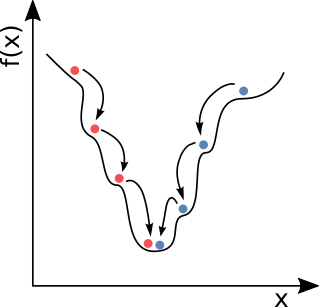
\includegraphics[width=.4\linewidth]{heightmap2a.png}
  	\label{subfig_hmap2ab:a}}\qquad
  \subbottom[]{
	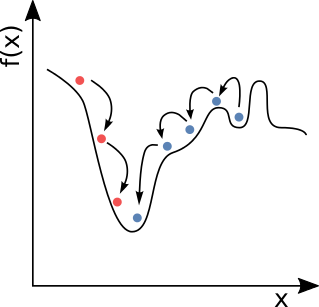
\includegraphics[width=.4\linewidth]{heightmap2b.png}
  	\label{subfig_hmap2ab:b}}
  \caption{Recherche d'un minimum global.}
  \label{fig:hmap2ab}
\end{figure}

En se limitant aux pièges dépendant de la topologie de l'espace des solutions \textcite[140]{Weise2011} a proposé un tableau synthétique de huits cas dont on extrait ici quelques exemples que l'on a modifié pour éclairer notre argumentaire.

On percoit bien sur ce schéma \ref{subfig_hmap2cd:c} quel effet peut avoir un déséquilibre entre les deux stratégies, une exploitation trop appuyée au détriment de l'exploration amenant souvent à une convergence prématurée, c'est à dire à un piège dans un optimum local. 

La figure \ref{subfig_hmap2cd:d} montre également que face à une topologie de fonction présentant un plateau relativement uniforme, l'optimiseur sera en peine pour trouver un minimum, même local. Un paramétrage différents de l'exploration pourra peut être résoudre ce problème, sans pour autant que l'on en soit sur. 

\begin{figure}[h]
  \centering
  \subbottom[]{
  	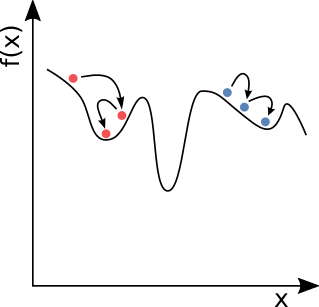
\includegraphics[width=.4\linewidth]{heightmap2e.png}
  	\label{subfig_hmap2cd:c}}\qquad
  \subbottom[]{
	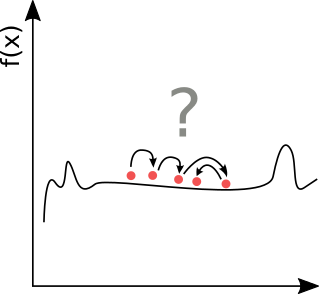
\includegraphics[width=.4\linewidth]{heightmap2c.png}
  	\label{subfig_hmap2cd:d}}
  \caption{Recherche d'un minimum global rendu plus difficile.}
  \label{fig:hmap2cd}
\end{figure}

Ce qui nous permet d'évoquer une faiblesse connu des métaheuristiques, hérité des remarques déjà faite sur les algorithmes d'optimisations stochastique \Anote{stochastic_note} dans laquelle on les place habituellement. La découverte garantie d'une solution globale optimale est en général difficile avec ce type d'algorithmes (cf. point \ref{enum_meta_d}) \Anote{equipe_mixite}, au moins pour deux raisons : 

\begin{enumerate}
\item la variabilité qui opère lors de la selection des solutions candidates à un instant $t$ ne permet pas de garantir qu'il n'existe pas quelque part une solutions candidate selectionné à $t+1$ dont l'évaluation révélera un meilleur optimum. La définition d'un critère d'arret est donc rendu délicate.
\item La variabilité dans l'établissement d'une trajectoire de recherche implique qu'un algorithme de même qualité puisse passer une première fois à coté d'un optimum, et une deuxième fois trouver celui-ci. 
\end{enumerate}

\begin{figure}[h]
  \centering
  \subbottom[]{
  	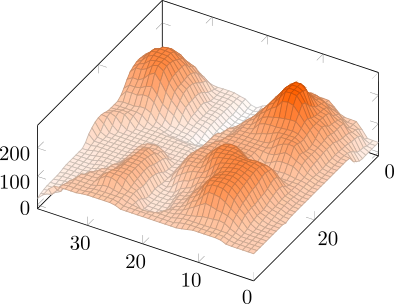
\includegraphics[width=.4\linewidth]{heightmap1a.png}
  	\label{subfig_hmap:a}}\qquad
  \subbottom[]{
	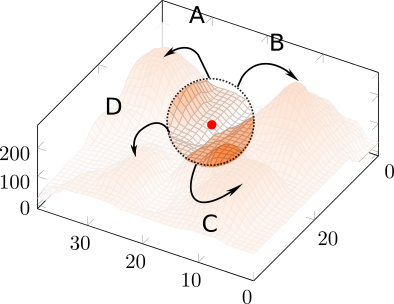
\includegraphics[width=.4\linewidth]{heightmap1b.png}
  	\label{subfig_hmap:b}}
  \caption{Navigation schématique d'une heuristique dans un espace de solution admettant deux types de valeurs résultat de l'évaluation.}
  \label{fig:hmap1}
\end{figure}

Pour mieux comprendre les problèmes posés par des espaces de solutions multi-modal, déjà figuré en deux dimensions dans \ref{subfig_hmap:b}, on représente cette fois ci dans la figure \ref{fig:hmap1} l'optimiseur dans un espace en trois dimensions, à la recherche d'un optimum global. La fonction ainsi représentée comporte deux entrées $x$,$y$, et une sortie $z = f(x,y)$ représentant la valeur numérique résultat de l'optimisation.

Attention à la lecture de ces schéma, il ne faut pas oublier que l'optimiseur \textbf{ne se déplace pas directement} sur le terrain visible dans la figure \ref{fig:hmap1}, et pour laquelle celui-ci n'a justement aucune visibilité. C'est un peu comme visualiser un labyrinthe de l'extérieur sur une feuille, puis de l'intérieur quand on s'y projette, la difficulté pour résoudre celui(ci n'est plus la même. La visibilité dont dispose l'optimiseur est celle des résultats de solutions candidates déjà évalués \ref{enum_meta_i} . Il s'agit donc de proposer de nouvelles solutions candidates soit en les composant à partir d'une manipulation des solution candidates déjà évalué, soit en introduisant de toutes nouvelles solution candidates prise de façon aléatoire. Au cours de l'itération mesurant la progression de l'algorithme, c'est bien l'évaluation de cette nouvelle population de solutions candidates qui détermine si il y'a effectivement eu un déplacement qualitatif dans l'espace des solutions. Le déplacement du point rouge dans l'espace des solutions n'est donc effectif que si on trouve à un instant $t + 1$ une solution plus intéressante qu'à l'instant $t$.

A partir des résultats de la première solution candidate évalué figuré ici en rouge dans \ref{fig:hmap1}, les opérateurs de recherches soumis à l'aléa d'une recomposition ou d'un tirage alétoire peuvent tout à fait proposer un candidat à $(x,y)_(t+1)$ qui débouche sur un résultat $z = f(x,y)$ placant l'optimiseur dans le sillon d'un gradient de pente parmi plusieurs. Ce qui ménera probablement l'optimiseur à découvrir des optimums de qualités très différentes : A (local) ,B (global) ,C (local) ,D (local). 

%Comment s'effectue la manipulation des opérateurs de recherches ? Comment opère le lien entre cet espace de recherche que les opérateurs de la métaheuristique manipule, et l'espace de solutions que l'on cherche à explorer ?
\hl{-- en cours de travail 31 janv --}

On revient à parler ici de l'heuristique, qui vient appuyer le choix de l'optimiseur par l'injection d'une connaissance externe, celle de l'expérimentateur.

De fait dans un tel scénario, et pour éviter une recherche aléatoire, l'évaluation de solution candidate renvoie à l'existence d'une expertise externe à l'optimiseur, le seul capable de formaliser ce qui différencie une bonne solution d'une mauvaise solution. 




% EXPERTISE enum_meta_h \ref{enum_meta_h} %

Une part d'expertise réside dans la maitrise du paramétrages des ces algorithmes d'optimisation, et dans la formulation de l'heuristique qui va le guider.

C'est l'injection de cette connaissance dans l'optimiseur qui va permettre à ce dernier de prendre les bonnes décisions quant au future solution candidates à évaluer dans ce processus de recherche forcément incrémental. On commence par l'évaluation de solution candidate au hasard, et petit à petit, du fait des opérateurs permettant la selection de nouvelle solution candidate, on espère voir émerger de meilleures solutions.

L'injection de connaissance dans ce type d'algorithme est donc double, et opère à la fois de façon précise dans la formalisation d'un ou de plusieurs critères qui vont servir pour l'algorithme optimiseur à déterminer la qualité, bonne ou mauvaise, d'une solution candidate; et de l'autre elle intervient cette fois ci de façon moins précise dans la façon dont l'expérimentateur va devoir choisir et paramétrer une métaheuristique pour l'adapter au mieux à son problème.

La qualité interne (paramètre, structure) de la métaheuristique définit aussi en quelque sorte le processus d'exploration, ce qui explique aussi la dépendance de ce type d'algorithmes à l'environnement qu'il doivent explorer.

Des tests mesurant la réponse de ces différents algorithmes d'optimisation ont étés formalisés ces dernières années, d'abord par la création de fonctions mathématiques \textit{benchmark} dont on connait la forme, ensuite par la mise en oeuvre de plateforme dédié à la confrontation entre ces algorithmes dans des workshop dédiés, comme la plateforme COCO (COmparing Continuous Optimisers) créé par Inra, et utilisé depuis 2009 pour les conférences GECCO.

Autrement dit, en plus de la stochasticité inhérente de ces algorithmes, non seulement un algorithme de type $A$ n'aura pas les même résultats qu'un algorithme de type $B$, mais celui sera également différent d'un algorithme $A'$ du fait d'un paramétrage différent.

Comme déjà évoqué dans la définition, on retrouve ici la qualité de flexibilité des métaheuristiques, permettant de transformer ce qui pourrait de prime abord paraitre pour un défaut, en qualité. 

Elle permettent de répondre plus aisément aux question suivantes \Anote{q_ppr} : 
\begin{enumerate}
\item  \foreignquote{english}{What parameter settings do I use to get good results when applying heuristic method X to problem Y?}
\item  \foreignquote{english}{How do I adjust the parameters of heuristic X so I get better results on problem Y?}
\item \foreignquote{english}{Which is \enquote{better}, heuristic X or heuristic Y?}
\end{enumerate}

Les métaheuristiques fournissent le support générique initial pour en fait un outil d'usage indépendant du problème, tout en fournissant les outils pour favoriser leur propre modification en vue d'une amélioration de résultat pour un problème donné. Elle cumule donc en quelques sorte les deux propriétés de dépendance et d'indépendance face à un problème donné. 

Mais la recherche ne se contente pas d'organiser une forme de compétition qui menerait à elle seule, par apprentissage des fonctions, à une surestimation de certains algorithmes, et se nourrit également d'une recherche plus appliqué à des problématique réelles. Ce qui permet par effet retour, d'espérer voir appliquer à des formes de problèmes génériques, des opérateurs dédiés à l'origine à des problèmatiques spécifiques. La construction et l'évaluation d'heuristique plus performante servant toujours indirectement une cause plus générale.

En résumé on pourrait dire qu'une \foreignquote{english}{metaheuristic is a pretty good rule for finding pretty good rules.}

%De part ce phénomène de \textit{sampling} et la façon dont on décide d'aborder le problème, l'horizon de connaissance d'une métaheuristique est donc assez limité, ce qui en fait sa force tout autant que sa faiblesse. 

% PAS BON





%S\textcite[225]{Weise2011} défini une métaheuristique sous le terme peut être moins ambigue d'une optimisation de type boite noire (\textit{black box optimization}, celle-ci étant une \foreignquote{english}{ [...] technique which combines information from the objective functions gained by sampling the search space in a way which (hopefully) leads to the discovery of candidate solutions with high utility}

Cette définition nécessite pour être comprise d'introduire de nouveaux éléments de définition caractérisant de façon générique et simplifié quel est la structure et la dynamique d'un problème d'optimisation.

\paragraph{Une formulation mathématique standardisé pour encadrer les problème d'optimisation}

%search space p 82
%structure p 101
% pareto ranking p 275

Pour comprendre comment se déroule de façon générale la résolution d'un problème d'optimisation, il faut poser un certain nombre de notions qui nous seront utiles par la suite. Cet exercice de description plus mathématique et générique s'appuie là encore principalement sur les écrits de \textcite{Weise2011}

La première étape selon Weise dans la construction d'un problème d'optimisation est de définir le type de structure qui peut être associée à l'expression des solutions possibles et spécifiques à notre problème.

Autrement dit, il s'agit de déterminer quel est l'espace dans lequel évolue la donnée figurant la solution attendue pour cette optimisation. L'expression de cette solution peut appartenir à l'espace des réels $\mathbb{R}$, comme par exemple une valeur numérique se rapportant à l'optimisation d'une fonction mathématique. Mais celle-ci peut également s'exprimer dans un repère beaucoup plus complexe, en faisant référence par exemple à un repère géométrique définissant le cadre  d'une forme à optimiser comme une pièce de moteur, une pièce d'avion, etc. \autocite[43]{Weise2011}

Cet espace du problème (\textit{problem space}) $\mathbb{X}$ est définit comme \foreignquote{english}{ [...] the set containing all elements $x$ which could be its solution.} 

Une solution candidate $x$ est quand à elle définit comme \foreignquote{english}{ [...] an element of the problem space $ \mathbb{X}$ of a certain optimization problem.}

L'objectif de l'optimisation est donc de trouver par le biais d'un algorithme adapté l'ensemble des solutions candidates $x^*$ appartenant à l'espace du problème répondant le mieux aux critères définis par l'utilisateur. Ce qui suppose de pouvoir qualifier une solution candidate $x_1$ tiré de $\mathbb{X}$ par rapport à une autre solution candidate $x_2$ elle aussi tiré de $\mathbb{X}$.

Une deuxième étape logique serait donc d'établir comment se fait la mesure établissant la qualité d'une solution ? 

Comme on pu la définir précédemment, ce qui va guider l'algorithme optimiseur dans sa prise de décision, c'est l'évaluation d'une fonction heuristique, ou d'une fonction objective (\textit{objective function}) \Anote{difference_objective_heuristique} 

\foreignquote{english}{An objective function $f: \mathbb{X} \mapsto \mathbb{R}$ is a mathematical function which is subject to optimization.}

Cette fonction objective lorsqu'elle prend pour paramètre un élément candidat $x$ pris dans l'espace du problème $ \mathbb{X}$ renvoie une valeur définissant sa qualité par rapport au problème posé. \autocite[44]{Weise2011}

La plupart des problèmes nécessite toutefois d'optimiser plusieurs critères simultanément. La relation entre ces critères peut d'ailleurs être elle aussi multiples : dépendante (conflictuelle, en harmonie), indépendante. Nous allons donc nous intéresser directement à la définition de ce type de problème, résumable ainsi : $min(f_1(x),\dotsc, f_k(x)$ avec $k > 2$

La littérature fait également plus souvent référence à ce type de problème en faisant appel à une notation sous forme de fonction vecteurs. Un ensemble $\vec{f} : \mathbb{X} \mapsto \mathbb{R^n}$ fait de $n$ fonction objective $f_i : \mathbb{X} \mapsto \mathbb{R}$ avec $\forall i \in 1 \dotsc n$. 

$\vec{f} : \mathbb{X} \mapsto \mathbb{R^n}$ renvoie un vecteur de réel de dimension $n$, $R^n$ renvoyant ainsi à l'espace des objectif (\textit{objective space}) $\mathbb{Y}$ quand cette fonction est appliqué à une solution candidate $x \in \mathbb{X}$ 

Autrement dit, à chaque association d'un vecteur de fonction objectif $\vec{f}$ et d'une solution candidate $x$ correspond après évaluation un vecteur de réel positionnant la solution candidate dans l'espace des objectifs $\mathbb{Y}$.

C'est à partir du positionnement des solutions candidates dans cet espace $\mathbb{Y}$ que l'optimiseur va décider de la prochaine solution candidate à évaluer. Dès lors, comment ce choix se fait-il dans une perspective multi-objectif à priori contradictoire ?

Si on considère par exemple la fonction multi-objective de Schaeffer décrite dans l'équation \ref{eq:schaffer}, $f1(x)$ and $f2(x)$ deux fonctions objectives à minimiser $ \vec{f} = (f1(x),f2(x))^T$  avec $\vec{f}: \mathbb{X} \mapsto \mathbb{R^2}$

\begin{equation} \label{eq:schaffer}
Minimize = 
	\begin{cases}
	 f1(x) = x^2 \\
	 f2(x) = (x-2)^2
	\end{cases}
\end{equation}

Si on superpose les deux fonctions comme dans la figure \ref{fig:S_Schaffer}, on voit bien qu'elles sont contradictoires, il s'agit donc de trouver un compromis.

\begin{figure}[h]

\begin{sidecaption}[fortoc]{ Pour la valeur $x = 0$, $f1(x) = 0 $ et $f2(x) = 4 $, pour $x = 2$,  $f1(x) = 4 $ et $f2(x) = 0 $ , donc la configuration inverse. La solution pour minimiser les deux fonctions $f1$ et $f2$ tient donc forcément dans un compromis dans la valeur prise par $x$.}[fig:S_Schaffer]
	\centering
 
	\begin{tikzpicture}[line cap=round,line join=round,>=triangle 45,x=1.0cm,y=1.0cm]
	\draw [color=cqcqcq,dash pattern=on 1pt off 1pt, xstep=1.0cm,ystep=1.0cm] (-5,-1) grid (5,5);
	\draw[->,color=black] (-5,0) -- (5,0);
	\foreach \x in {-5,-4,-3,-2,-1,1,2,3,4}
	\draw[shift={(\x,0)},color=black] (0pt,2pt) -- (0pt,-2pt) node[below] {\footnotesize $\x$};
	\draw[->,color=black] (0,-1) -- (0,5);
	\foreach \y in {-1,1,2,3,4}
	\draw[shift={(0,\y)},color=black] (2pt,0pt) -- (-2pt,0pt) node[left] {\footnotesize $\y$};
	\draw[color=black] (0pt,-10pt) node[right] {\footnotesize $0$};
	\clip(-5,-1) rectangle (5,5);
	\draw[color=ttttff] plot[raw gnuplot, id=func2] function{set samples 100; set xrange [-4.9:4.9]; plot x**2};
	\draw[color=fftttt] plot[raw gnuplot, id=func3] function{set samples 100; set xrange [-4.9:4.9]; plot (x-2)**2};
	\begin{scriptsize}
	\draw[color=ttttff] (-2.26,6.14) node {$f$};
	\draw[color=fftttt] (-0.24,6.14) node {$g$};
	\end{scriptsize}
	\end{tikzpicture}
 \end{sidecaption}
\end{figure}

En réalité l'optimiseur n'a pas vraiment les moyens de comparer des fonctions entre elle, et doit bien en définitive attribuer un scalaire caractérisant chaque vecteur $z^* \in \mathbb{Y}$ résultat de l'évaluation d'une solution candidate afin de guider l'optimisation. Dans le cas d'un problème multi-objectif, la stratégie de comparaison la plus efficace et la plus courrament utilisé pour déterminer de cette valeur est probablement celle du \foreignquote{english}{Pareto ranking}. 

Cette opération que nous pratiquons tout les jours sans le savoir peut être plus facilement expliqué en faisant appel à cet exemple concret. Dans le cas d'un acheteur à la recherche d'une voiture à la fois économe de par sa faible consommation et si possible disponible à un moindre cout, celui ci devra bien se plier à l'exercice de positionnement des voitures résumé dans le graphique \ref{fig:voiture}. 

\begin{figure}[h]
  \centering
  \subtop[]{
  	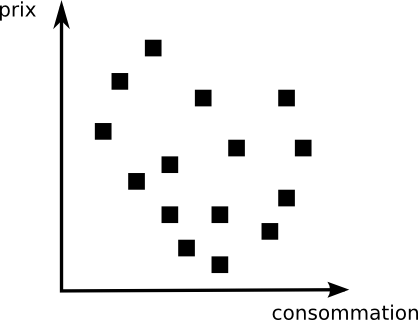
\includegraphics[width=.3\linewidth]{opti1.png}
  	\label{subfig_voiture:a}}\qquad
  \subtop[]{
	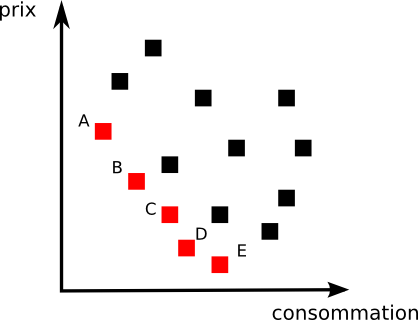
\includegraphics[width=.3\linewidth]{opti2.png}
  	\label{subfig_voiture:b}}
  \subtop[]{
  	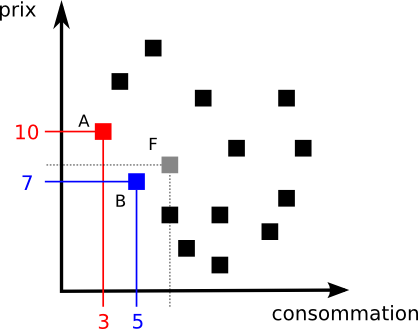
\includegraphics[width=.3\linewidth]{opti3.png}
  	\label{subfig_voiture:c}}
  \caption{Exemple simplifié d'une catégorisation de voitures selon deux axes comprenant d'une part le cout d'achat et d'autre part la consommation de chaque voiture}
  \label{fig:voiture}
\end{figure}

Dans le graphique \ref{subfig_voiture:b} on constate rapidement que le modèle de voiture que l'acheteur va acheter à de forte chance de se trouver dans la liste de voiture ${A,B,C,D,E}$ coloré en rouge, aussi appelé front de Pareto, ou optimum de Pareto.

En regardant en détail les capacités des voitures figurant dans ce front \ref{subfig_voiture:c}, on voit bien que chacune d'entre elle domine une partie des autres voitures sur au moins un des deux objectifs. Si on prend le cas de la voiture F, celle ci n'est pas dans le front car il est dominé sur ces deux objectif par d'autre voitures $ prix(B) < prix(F) < prix(A) $ et consommation $consommation (A) < consommation(B) < consommation(F)$.

Le front de pareto renvoie un ensemble de solutions compromis, l'expertise finale sur la ou les solutions à adopter est donc un choix expert externe à l'algorithme optimiseur. Dans notre exemple, l'acheteur devra pour finaliser son achat mettre en avant au moins un des deux critères afin de départager les voitures.

\hl{-- en cours 22 janv --}



Première fois utilisé en 1989

Si on transfère ce langage neutre au vocabulaire que l'on peut trouver courrament dans l'EC, alors l'espace des solution devient le \textit{phenome}, et le point de cet espace qui correspond à la solution candidate devient un \textit{phenotype}.

%\begin{figure}
%\begin{sidecaption}[fortoc]{ POM cycle for developping theory for an agent behavior \autocite[245]{Railsback2012}}[fig:S_syntheseGrim]
%  \centering
% 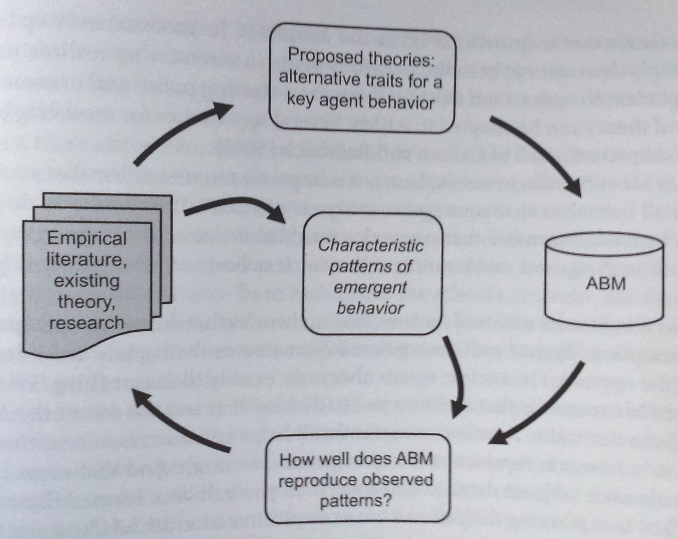
\includegraphics[width=.9\linewidth]{cyclePOMcomportement.png}
%  \end{sidecaption}
%\end{figure}

Il faut bien comprendre que cette mesure d'utilité, ou fitness, est calculé de façon indépendante de la fonction objectif, par rapport aux positionnements des autres solutions.



Dans notre étude, l'objet à optimiser ne se réfère pas à une expression mathématique, mais à un modèle de simulation, sur lequel on va déterminer un ensemble de critères qui vont faire figure d'équivalent de ces fonction objectives. Dans ce cas d'utilisation, l'optimisation est plus souvent employé comme une forme de calibration inversé \autocite{Grimm2011}, dans laquelle on cherche à déterminer si il existe un ou plusieurs jeu de valeur de paramètres du modèles de simulation respectant la plage de valeur viable empiriquement qui permettent de maximiser l'obtention d'un ou de plusieurs critères experts. 


Il est plus parlant dans notre cas de désigner l'espace de recherche comme l'espace des paramètres.  

 il s'agit pour nous de trouver qu'elles sont les valeurs de paramètres optimales compte tenu des critères fixés pour qualifier de la réussite d'une simulation. Ces critères dont l'inter-relation est variable (indépendance, dépendance, etc.) constituent un lot de fonctions objectives dont la résolution passe par l'execution de notre simulation.

The search space $\mathbb{X}$ (genome) of an optimization problem is the set of all elements $g$ which can be processed by the search operations.

109 - 111

Une opération de projection permet de passer de l'espace de recherche à l'espace des problèmes. C'est ce que Weise2011 appelle le Genotype-Phenotype mapping. 


L'espace du problème $\mathbb{X}$ (\textit{problem space}), l'espace de recherche $\mathbb{G}$ (\textit{search space}) et l'opération de transformation qui permet de passer de l'espace de recherche à l'espace du problème (

Une des premières étapes est de considérer la nature prises par ces deux espaces.

In single-objective optimization, it means to find the candidate solutions which lead to either minimum or maximum objective values. In multi-objective optimization, there exist a variety of approaches to define optima which we will discuss in-depth in Section 3.3.

In a multi-objective optimization problem (MOP), a set f : X 7→ R n consisting of n objective functions f i : X 7→ R, ea

\subsubsection{Rappel historique de la discipline}

On a déjà rapidement décrit dans la section à propos de l'Artificial Life \ref{p:heritage_complexe} les deux voies qu'il était possible d'emprunter dans l'intéret porté sur la définition du processus naturel d'évolution. 

Il existe en effet au moins deux façons aujourd'hui d'introduire des développements informatiques se rapportant à ce processus évolutif. D'un côté, les tentatives de reproduction plus ou moins fidèles des différents mécanismes à l'oeuvre dans le processus d'évolution mettent en avant un objectif de compréhension, alors que la focalisation sur ces mêmes mécanismes pour leur seule capacité d'apprentissage tend à s'éloigner de la réalité biologique pour s'orienter plus vers le développement d'algorithmes désignés comme métaheuristiques. Autrement dit, là ou des chercheurs vont tenter de reproduire au mieux le processus d'évolution dans ce qu'il a de créatif, de non optimisé, de coévolutif car construit par \Anote{note_pattee_semantic_closure} et avec l'environnement, d'autres vont reprendre ce même processus en vue d'une évolution si possible bornée et dirigée par la résolution efficace d'un ou de plusieurs objectifs définis de façon fixe et extrinsèque \autocites{Taylor2001, Taylor2012}.

Lorsqu'on s'intéresse de plus près à la littérature scientifique de ces algorithmes regroupés depuis Fogel sous le terme d'\foreignquote{english}{Evolutionary Computation} (EC), on constate pour toute une partie des publications une de-contextualisation complète de leur utilisation. La question d'une similitude initiale avec le vivant n'étant le plus souvent évoquée que pour illustrer des racines historiques éloignées. Ce qui peut apparaitre comme une forme de surspécialisation est en quelques sortes le prix à payer d'une évolution de la discipline avant tout dirigée par une communauté de chercheurs informatiques motivés par la recherche d'algorithmes performants et d'applications génériques.

Si aujourd'hui on peut observer un tel cloisonnement, un regard sur l'histoire de la discipline tend à montrer tout l'inverse, car nombreux sont les pionniers ayant développé des intérêts simultanés pour ces deux approches : les expériences très longtemps restées inconnue du mathématicien Barricelli dès 1954 \Anote{barricelli_multi_utilisation}, l'approche du généticien \textcite{Fraser1957} qui décrit et simule l'évolution de population génétique dès 1957 \Anote{fraser_comment}, les travaux de Pattee et Conrad avec EVOLVE à la fin des années 1960 \autocite{Conrad1970}, les algorithmes génétiques \Anote{holland_multi_utilisation} de Holland, un disciple de Burks.

Il existe toutefois une littérature scientifique parallèle qui continue de motiver la rencontre autour de disciplines scientifiques ayant un intérêt pour la recherche en \textit{Artificial Life}. C'est le cas par exemple de la biologie, ou de l'écologie \autocite{Hamblin2013} qui organisent autour de publications transverses la réflexion sur la reintroduction des outils tel qu'ils sont développés en informatique, entrainant de fait aussi la création et l'évolution de ces derniers \autocite{Hogeweg2011}. C'est également le cas en biologie, ou on imagine l'importance que peuvent avoir les travaux de \textcites{Taylor2001}[221]{Taylor1999} pour la mise en oeuvre de modèles de simulation dirigés vers l'émergence \enquote{créative} de nouveaux phénotypes dans un environnement ouvert \autocite[33]{Taylor1999}. Une critique récurrente adressée aux modèles d'auto-organisation actuels \autocite{Pumain2003}, encore incapables de simuler l'émergence de nouvelles structures, de nouvelles entités de façon crédible. Une autre forme de relation entre les deux approches est également envisageable dans certaines disciplines, comme en écologie, où celles-ci peuvent parfaitement se côtoyer : \foreignquote{english}{The first of these requires the application of the evolutionary process in much the same way as it has been traditionally applied within A-Life: as a means to dynamically adjust agent parameter values to support their viability and reproduction within the virtual environment. [...] The second approach we suggest employs artificial evolution to match simulation patterns against data gathered from the level of specific species up to data concerning specific ecosystems. Once the parameters of the system have been optimised so as to reproduce the patterns observed in field data, the evolution algorithm is turned off. The model may then be employed to answer questions relating to the specific ecosystem and species that it represents. Unfortunately it may not then be used to study the evolution of these specific species in specific environments. This is a shortcoming of the artificial evolution algorithm (it does not model real evolution in detail) that would be worth overcoming.} \autocite{Dorin2008}

On trouve plus de détails sur l'histoire communes de ces deux voies de recherches du point de vue de l'EC dans les ouvrages de \autocites{DeJong2006a, Fogel1998, Fogel2006a, Fogel2006b}. \hl{ et Back1997 ?} 

Dans ce chapitre, c'est bien la deuxième branche de recherche qui est suivie, celle visant l'\enquote{optimisation}. Les développements tels qu'ils sont abordés ne se mesurent donc plus en fonction d'un critère de réalisme biologique, mais en fonction de critères informatiques et mathématiques se rapportant plus à la capacité de résolution des algorithmes, et aux supports de mise en oeuvre de ces derniers : rapidité, diversité, robustesse, etc.

\textcite{DeJong2006a} retient trois foyers importants pour le développement de cette deuxième branche dans les années 1960, la \textit{Technical University} de Berlin avec Rechenberg et Schwefel, UCLA à la même période avec Lawrence J. Fogel, et l'université du Michigan avec John Holland.

De ces trois branches vont émerger au cours des années 1970 ce que \textcite{DeJong2006a} qualifie de \foreignquote{english}{Evolutionary Algorithms (EA)} canoniques. Autrement dit, ce sont des algorithmes matures, qui ont prouvé leur capacité à produire des solutions dans un contexte précis : \foreignquote{english}{Evolutionary Programming (EP)}, \foreignquote{english}{Evolution Strategy (ES)}, \foreignquote{english}{Genetic Algorithm (GA)}

Ils vont représenter chacun le foyer d'un développement qui va s'accélérer dans les années 1980, avec l'amorce d'une popularisation de ces techniques permises entre autres par l'avènement de capacités de calcul plus conséquentes et la reconnaissance de l'efficacité de ces algorithmes pour la résolution de problématiques industrielles plus concrètes \autocite{Goldberg1989}. Les années 1990 vont quant à elles consacrer la rencontre et l'unification de ces différentes approches restée jusqu'alors assez indépendantes si on en croit \textcite{DeJong2006a}. De cette confrontation nait la reconnaissance d'un seul terme fédérateur, l'\textit{Evolutionary Computation (EC)} motivant alors la création de nouvelles conférences et de nouveaux journaux structurant cette nouvelle discipline. C'est aussi à partir de cette période que l'on observe une hybridation accélérée entre les différentes approches et une forme de remise à plat théorique qui passe on va le voir plus tard par la définition d'un cadre commun. \autocites[23-31]{DeJong2006a}{Back1997}

Enfin on notera qu'il existe également une autre classe proche d'algorithmes d'optimisation basée sur une observation des mécanismes naturels, celle-ci n'étant plus basée sur la métaphore évolutive par reproduction (même si l'hybridation est envisageable), mais sur les capacités d'organisation et d'auto-organisation observées chez certains animaux comme les fourmis, les abeilles. Ces comportements ont d'abord inspiré les développements de plateformes informatiques adaptées à l'émergence de ce type de comportements, avant d'être repris et utilisé de façon beaucoup plus abstraites par la suite pour résoudre des problèmes d'optimisation. Aujourd'hui regroupées sous le terme de \foreignquote{english}{Swarm Intelligence}, ce sont par exemple les algorithmes PSO (Particle Swarm Optimization), ACO (Ant Colony Algorithms), ABC (Artificial Bee Colony), etc.


\subsubsection{Terminologie et concept clef spécifique à l'EC}

En 2014 une publication sur le blog du spécialiste de la discipline Thomas Weise's \Anote{billet_weise} revient longuemment sur les problématiques de ce vocabulaire inspiré par la biologie et ancré dans les différentes branches composantes l'EC. Il retient quatre problématiques dans l'usage de cette terminologie, parmi lesquels l'incompatibilité des terminologies entre les différentes branches, la dissonance entre la terminologie et la réalité d'application des algorithmes, le fait que l'optimisation au sens naturel n'est pas forcément une bonne optimisation,  le fait également que cette terminologie sonne comme anti-profesionelle \Anote{note_pengouin} Le plus grand problème étant dans ce cadre l'invention de néologisme ne faisant référence ni au domaine biologique, ni au domaine informatique.

Si la perspective d'un changement d'annotation et de vocabulaire est probablement conçu comme une étape majeure dans la progression et l'unification d'une discipline depuis quelques années déjà sur la voie de la maturité, Weise tout en pronant au maximum la bonne parole continue comme beaucoup d'autres à utiliser cette terminologie, très ancré dans un folklore qui tient à l'historique de la discipline. La librairie logicielle MGO décrite par la suite s'appuie sur cette terminologie, ainsi nous n'utiliserons donc les terminologies alternatives proposés par Weis que sous forme de complétement, afin de ne pas introduire trop de distance entre les termes décrivant les algorithmes dans ce manuscrit et la réalité du programme conçu.

\hl{Principe général}

Afin de pouvoir mettre en oeuvre la possibilité d'une telle souplesse dans l'adaptation de l'algorithme à une problématique d'optimisation donnée, il a considérer la construction d'un modèle conceptuel plus abstrait capable d'englober dans sa description les mécanismes d'au moins ces trois version canoniques. Les concepts clef qui se dégagent d'une telle prise de distance peuvent ainsi être repris non seulement pour décrire les version canoniques mais également pour développer de nouvelles variantes ou extensions d'algorithmes.

\textcite{DeJong2006a} propose de retenir dans un cadre de construction commun le schéma d'éxecution suivant : 

\begin{itemize}
\item Une population de taille constante $m$ évolue au cours du temps
\item La population courante est utilisé comme une source de parents pour produire une progéniture de taille $n$
\item La population étendue ainsi constitué est réduites de $m + n$ à $m$ individus.
\end{itemize}

Les classes d'élements amenés à varier sont ainsi les suivantes : 

\begin{itemize}
\item une population de taille m
\item une progéniture de taille n
\item une méthode de selection des parents
\item une méthode de selection des survivants
\item un ensemble d'opérateurs pour la reproduction
\item une méthode interne pour la représentation des individus
\end{itemize}

$g := 1$ to $G_{max}$

\begin{algorithm}[H]
 \KwData{this text}
 \KwResult{how to write algorithm with \LaTeX2e }
 initialization\;
 \While{not at end of this document}{
  read current\;
  \eIf{understand}{
   go to next section\;
   current section becomes this one\;
   }{
   go back to the beginning of current section\;
  }
 }
 \caption{How to write algorithms}
\end{algorithm}

((Schéma))

A partir d'une description minimale et communément accepté de ce processus ont dérivés de nouveaux blocs, et de nouveaux schéma d'organisation

La modularité de cette architecture a déjà pu par chance être saisie dans le développement de librairies logicielles 


Les librairies logicielles permettant la mise en oeuvre d'algorithmes évolutionnaires existent dans de très nombreux langages informatiques.


\subsection{Quelle utilité pour la construction et l'évaluation de modèle de simulation ?}


\subsection{Conception et Implémentation d'une nouvelle librairies}

\subsubsection{Un point rapide sur les nombreuses librairies existantes}

\subsubsection{La nécessité d'une librairie couplé avec la modélisation}

\begin{itemize}
	\item Une architecture extensible et modulaire
	\item Une mise en oeuvre accessible aux débutants
	\item Une prise en charge automatique et transparente des architecture multi-coeur 
	\item La mise à disposition d'une collection d'algorithmes evolutionnaire mono et multi-critères 
\end{itemize}

Mais si on se contente d'évoquer seulement ces objectifs là, on reste dans une construction isolé dont il faut encore l'interfacer, la relier, à l'execution de nos modèles de simulation.

La généricité d'application de cette librairie à différentes classes de problèmes tient dans la sémantique associé à chacun des éléments de la terminologie. 

Dans notre étude, les \textit{individus} représentent une instance de simulation,



\paragraph{BehaviorSearch}

La librairie \textit{BehaviorSearch} developpé par Railsback pour Netlogo intègre une librairie d'algorithme génétique.

\paragraph{MGO et OpenMOLE}

Le choix est fait ici de développé une librairie MGO utilisable de façon indépendante, ou de façon couplé à openMOLE. 

Les objectifs motivant la construction d'une nouvelle librairie sont les suivants : 



L'étape suivante est donc le couplage de cette librairie avec openMOLE 


- La possibilité d'utiliser des algorithmes génétique avec une grille de calcul


Martin Oderskys’


\begin{minted}[linenos=true,frame=single,fontsize=\footnotesize]{scala}
import fr.iscpif.mgo._
import math._
import util.Random

trait ZDT4 extends GAProblem with MGFitness {

  def min = Seq.fill(genomeSize)(0.0)
  def max = 1.0 :: Seq.fill(genomeSize - 1)(5.0)

  type P = Seq[Double]

  override def express(g: Seq[Double], rng: Random) = Seq(f1(g), f2(g))
  override def evaluate(p: P, rng: Random) = p

  def f1(x: Seq[Double]) = x(0)
  def f2(x: Seq[Double]) = g(x) * (1 - sqrt(x(0) / g(x)))
  def g(x: Seq[Double]) =
    1 + 10 * (genomeSize - 1) + (1 until genomeSize).map 
    { i => pow(x(i), 2) - 10 * cos(4 * Pi * x(i)) }.sum
}
}
\end{minted}

\subsection{Une brique logicielle dédiée à la visualisation de résultats}


